\documentclass[12pt,titlepage]{article}
\usepackage[margin=1.25in]{geometry}
\usepackage{graphicx,amsmath,blindtext,minted}

%% Variables definition
\newcommand{\vSubject}{Advandce Database}
\newcommand{\vSubtitle}{Intro to TSQL and TSQL Statement}
\newcommand{\vName}{Muhammad Baihaqi Aulia Asy'ari}
\newcommand{\vNIM}{2241720145}
\newcommand{\vClass}{2I}
\newcommand{\vDepartment}{Information Technology}
\newcommand{\vStudyProgram}{D4 Informatics Engineering}

%% [START] Tikz related stuff
\usepackage{tikz}
\usetikzlibrary{svg.path,calc,shapes.geometric,shapes.misc}
\tikzstyle{terminator} = [rectangle, draw, text centered, rounded corners = 1em, minimum height=2em]
\tikzstyle{preparation} = [chamfered rectangle, chamfered rectangle sep=0.75em, draw, text centered, minimum height = 2em]
\tikzstyle{process} = [rectangle, draw, text centered, minimum height=2em]
\tikzstyle{decision} = [diamond, aspect=2, draw, text centered, minimum height=2em]
\tikzstyle{data}=[trapezium, draw, text centered, trapezium left angle=60, trapezium right angle=120, minimum height=2em]
\tikzstyle{connector} = [line width=0.25mm,->]
%% [END] Tikz related stuff

%% [START] Fancy header related stuff
\usepackage{fancyhdr}
\pagestyle{fancy}
\setlength{\headheight}{15pt} % compensate fancyhdr style
\fancyhead{}
\fancyfoot{}
\fancyfoot[L]{\thepage}
\fancyfoot[R]{\textit{\vSubject - \vSubtitle}}
\renewcommand{\footrulewidth}{0.4pt}% default is 0pt, overline for footer
%% [END] Fancy header related stuff

%% [START] Custom tabular command related stuff
\usepackage{tabularx}
\newcommand{\details}[2]{
    #1 & #2  \\
}
%% [END] Custom tabular command related stuff

%% [START] Figure related stuff
\newcommand{\image}[3][1]{
    \begin{figure}[h]
        \centering
        \includegraphics[#1]{#2}
        \caption{#3}
        \label{#3}
    \end{figure}
}
%% [END] Figure related stuff

%%
\usepackage{pgf-umlcd}

\renewcommand{\umldrawcolor}{black}
\renewcommand{\umlfillcolor}{white}
%%

%% [BEGIN] Custom enumerator
\usepackage{enumitem}
%% [END] Custom enumerator

%% [BEGIN] Paragraph indent
\usepackage{indentfirst}
%% [END] Paragraph indent

\begin{document}
\begin{titlepage}
    \centering
    \vfill
    {\bfseries\LARGE
        \vSubject\\
        \vskip0.25cm
        \vSubtitle
    }
    \vfill
    
\includegraphics[width=6cm]{images/polinema-logo.png}
    \vfill
    {
        \textbf{Name}\\
        \vName\\
        \vskip0.5cm
        \textbf{NIM}\\
        \vNIM\\
        \vskip0.5cm
        \textbf{Class}\\
        \vClass\\
        \vskip0.5cm
        \textbf{Department}\\
        \vDepartment\\
        \vskip0.5cm
        \textbf{Study Program}\\
        \vStudyProgram
    }
\end{titlepage}

\newpage

\begin{enumerate}
    \section*{Practicum - Part 1}
    \item The difference is that the first query select every part using the wildcard symbol and the second query declared every column to be displayed sequentially
    \section*{Practicum - Part 2}
    \item Yes, because the query ask for the data in column country on every row. \\
    \includegraphics[height=.76\textheight]{images/figures/fig1.png}
    \newpage
    \item No, the difference is how the 4th step query result is unique and there is no duplicate data. From the experiment it can be concluded that the DISTINCT keyword is used to query data without any duplicate data. \\
    \includegraphics[height=.8\textheight]{images/figures/fig2.png}
    \newpage
    \section*{Practicum - Part 3}
    \item The column name of the query is different. The AS keyword is used to make an alias to the name of the table and column such that you can represent the table/column with the alias declared with the AS keyword. \\
    \resizebox{.9\textwidth}{!}{
        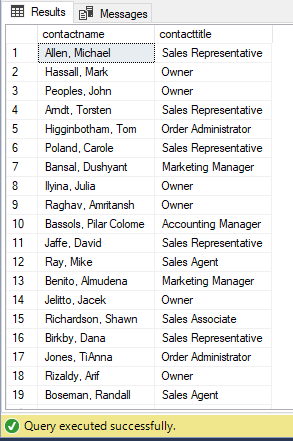
\includegraphics[height=\textheight]{images/figures/fig3_a.png}
        \includegraphics[height=\textheight]{images/figures/fig3_b.png}
    }
    \newpage
    \section*{Practicum - Part 4}
    \item step 3 query has an extra column of category name. CASE keyword seems to work like switch case, for multiple similar condition to output different result. \\
    \resizebox{.9\textwidth}{!}{
        \includegraphics[height=\textheight]{images/figures/fig4_a.png}
        \includegraphics[height=\textheight]{images/figures/fig4_b.png}
    }
    \newpage
    \item An extra column detailing if the product is a champaign product or not\\
    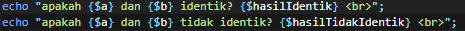
\includegraphics[width=.9\textwidth]{images/figures/fig5.png}
    \newpage
    \item 12 row affected
    \begin{minted}[autogobble,breaklines,linenos]{sql}
        SELECT
        p.categoryid , p.productname,
            CASE
                    WHEN p.categoryid = 1 THEN 'Beverages'
                    WHEN p.categoryid = 2 THEN 'Condiments'
                    WHEN p.categoryid = 3 THEN 'Confections'
                    WHEN p.categoryid = 4 THEN 'Dairy Products'
                    WHEN p.categoryid = 5 THEN 'Grains/Cereals'
                    WHEN p.categoryid = 6 THEN 'Meat/Poultry'
                    WHEN p.categoryid = 7 THEN 'Produce'
                    WHEN p.categoryid = 8 THEN 'Seafood'
                    ELSE 'Other'
            END AS categoryname,
            CASE
                    WHEN p.categoryid IN (1, 7, 8) THEN 'Champaign Products'
                    ELSE 'Non-Champaign Products'
            END AS iscampaign
        FROM [Production].[Products] AS p
        WHERE p.categoryid = 8;
    \end{minted}
    \resizebox{.9\textwidth}{!}{
        \includegraphics[height=\textheight]{images/figures/fig6_a.png}
        \includegraphics[height=\textheight]{images/figures/fig6_b.png}
    }
    \newpage
    \item -
    \begin{minted}[autogobble,breaklines,linenos]{sql}
        SELECT
            h.firstname AS FIRST_NAME,
            h.lastname AS LAST_NAME,
            h.city AS CITY,
            h.country AS COUNTRY
        FROM [HR].[Employees] AS h
        WHERE h.city = 'Seattle' AND h.country = 'USA';
    \end{minted}
    \section*{Practicum - Part 5}
    \item -
    \begin{minted}[autogobble,breaklines,linenos]{sql}
        [custid], [companyname], [contactname], [address], [city], [country], [phone]
        FROM Sales.[Customers]
        WHERE
        [country] = N'Brazil' OR
        [country] = N'UK' OR
        [country] = N'USA';
    \end{minted}
    \item -
    \begin{center}
        \includegraphics[height=.45\textheight]{images/figures/fig8.png}
    \end{center}
\end{enumerate}

\end{document}